\noindent
Para la realización de la tarea 1, se propone una red, para la cual se hace uso de GNS3, en donde se establecen 5 routers, así como otros dispositivos como computadora o túneles UDP.
\newline
A continuación, se muestra un diagrama con la topología propuesta:

\begin{figure}[htbp!]
	\centering
	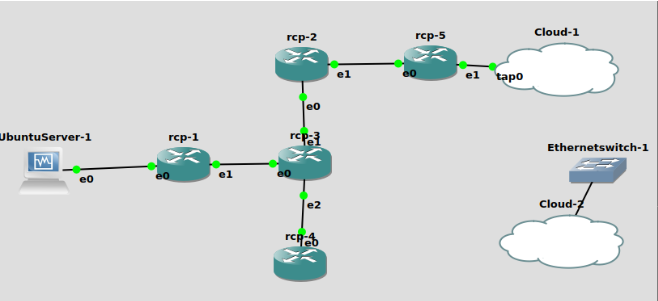
\includegraphics[width=1\textwidth]{desarrollo/tarea1/img/T1_img1}
	\caption{Topología propuesta.}
\end{figure}

\noindent
Así, una vez realizada la topología previamente mostrada, se procede a realizar en enlace y enrutamiento de cada nodo, para ello se hace uso de enrutamiento estático, o de protocolos como RIP y OSPF. Debajo se muestra un ejemplo de configuración para uno de los routers, haciendo uso del protocolo de enrutamiento RIP.
\newline

\noindent
en
\newline
conf
\newline
hostname R2
\newline
interface ethernet eth0
\newline
ip address 192.168.2.1/24
\newline
no sh
\newline
exit
\newline
interface ethernet eth0
\newline
ip address 192.168.4.1/24
\newline
no sh
\newline
exit
\newline
router rip
\newline
network 192.168.2.1/24
\newline
network 192.168.4.1/24
\newline
redistribute connected
\newline
exit
\newline
\newline
Así, una vez realizada la configuración de cada router en la topología con los protocolos mencionados, podemos ver los siguientes resultados en las tablas de enrutamiento de los routers R2, R3 y R4, en donde podemos observar la forma en que las rutas están distribuidas y la forma en que logran comunicar a los routers participantes. 

\begin{figure}[htbp!]
	\centering
	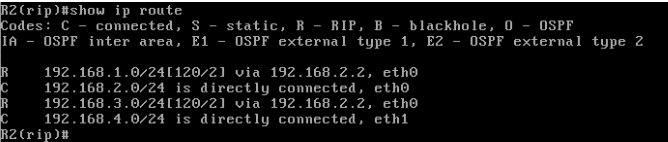
\includegraphics[width=1\textwidth]{desarrollo/tarea1/img/T1_img2}
	\caption{Tabla de enrutamiento del Router 2 (R2).}
\end{figure}

\begin{figure}[htbp!]
	\centering
	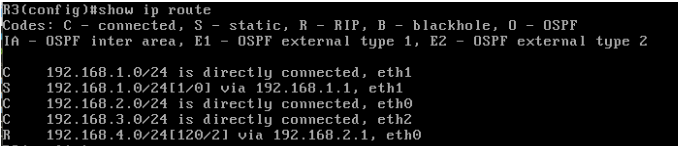
\includegraphics[width=1\textwidth]{desarrollo/tarea1/img/T1_img3}
	\caption{Tabla de enrutamiento del Router 3 (R3).}
\end{figure}

\pagebreak
\begin{figure}[htbp!]
	\centering
	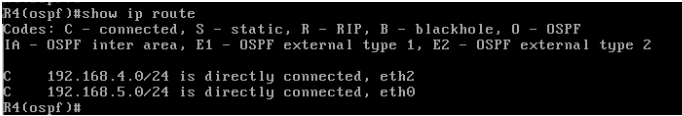
\includegraphics[width=1\textwidth]{desarrollo/tarea1/img/T1_img4}
	\caption{Tabla de enrutamiento del Router 4 (R4).}
\end{figure}

\noindent
Finalmente, se realizan pruebas de conexión entre los dos extremos de la red (UbuntuServer y Cloud) para verificar que la topología ha sido conectada y configurada correctamente. Para ello se hacen pings de extremo a extremo en ambas direcciones, los resultados pueden verse debajo. 

\begin{figure}[htbp!]
	\centering
	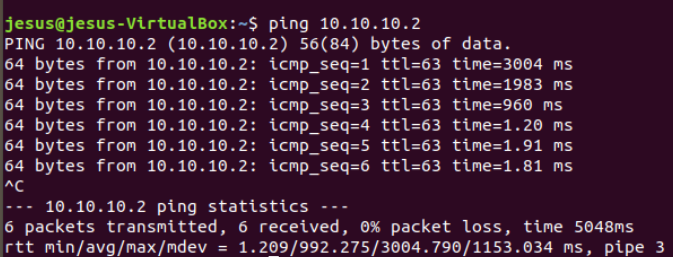
\includegraphics[width=1\textwidth]{desarrollo/tarea1/img/T1_img5}
	\caption{Ping de extremo 1 a extremo 2.}
\end{figure}

\begin{figure}[htbp!]
	\centering
	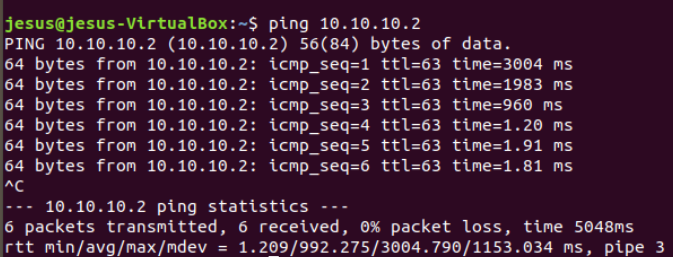
\includegraphics[width=1\textwidth]{desarrollo/tarea1/img/T1_img5}
	\caption{Ping de extremo 2 a extremo 1.}
\end{figure}